\documentclass[11pt]{article}

% Define margins
\usepackage{geometry}
\geometry{top=2cm, bottom=2cm, left=2cm, right=2cm, headheight=23pt}

\usepackage{graphicx}
\graphicspath{{images/}{../figures/}{figures/}}
\usepackage{float}
\usepackage[colorlinks=true, linkcolor=black, citecolor=black, urlcolor=blue]{hyperref}
\usepackage{subcaption}
\usepackage{booktabs}
\usepackage{tabularx}
\usepackage{multirow}
\usepackage{array}
\usepackage{algorithm}
\usepackage{algpseudocode}

% Header and footer
\usepackage{fancyhdr}
\pagestyle{fancy}
\fancyhf{}
\lhead{{\includegraphics[height=.65cm]{images/Logo_UPC.svg.png}}}
\rhead{\textbf{\textit{Computational Intelligence}}}
\cfoot{\textbf{\textit{\thepage}}}
\renewcommand{\headrulewidth}{0.7pt}

\usepackage{amsmath,amssymb,bm}
\usepackage[utf8]{inputenc}
\usepackage{enumitem}
\usepackage{xcolor}
\usepackage{microtype}
\usepackage[skip=10pt plus1pt, indent=20pt]{parskip}

% References
\usepackage{natbib}

% Macros
\newcommand{\cmaes}{CMA-ES}
\newcommand{\lbfgs}{L-BFGS-B}
\newcommand{\nfloor}{\sigma^2}
\newcommand{\clean}{\mathrm{MSE}_{\mathrm{clean}}}
\newcommand{\B}{B}
\newcommand{\Ltr}{L_{\mathrm{train}}}

\begin{document}

% Title Page %%%%%%%%%%%%%%%%%%%%%%%%%%%%%%%%%%%%%%%%%%%%%%%%%%%%%%%%%%%%%%%%%%%%%

\begin{center}

\includegraphics[width=1\textwidth]{images/logo.jpg}\\
\vfill

{\huge \textbf{Do Evolutionary Algorithms Generalise Better? A Controlled Comparison with Gradient-Based Methods Under Data Scarcity}}

\vspace*{3\baselineskip}

{\LARGE \textbf{Computational Intelligence final project}}

\begin{large}
\vspace*{2\baselineskip}

12/11/2026

\vspace*{2\baselineskip}

\emph{Students} \\[1ex]
{\Large Aram Abrahamyan\par}
{\Large Marta Mateu López\par}
\vspace*{2\baselineskip}
\emph{Teacher} \\[1ex]
{\Large Lluís A. Belanche \\ \par}
\vspace*{2\baselineskip}

\vspace*{4\baselineskip}

{Facultat d'Informàtica de Barcelona}\\
{\large Universitat Politècnica de Catalunya}\par

\thispagestyle{empty}

\end{large}
\end{center}
\pagebreak

% Contents %%%%%%%%%%%%%%%%%%%%%%%%%%%%%%%%%%%%%%%%%%%%%%%%%%%%%%%%%%%%%%%%%%%%%%%

\newpage
\pagenumbering{roman}
\tableofcontents
\cleardoublepage
\pagenumbering{arabic}

% ============================================================
\section{Introduction}
% ============================================================

The application of evolutionary search to artificial neural networks is a long-standing research topic
\citep{yao1999evolving}. Evolution can act on the connection weights, the architecture, the
hyper-parameters, the activation functions and the learning rules. For weight training, EAs have clear
advantages over derivative-based methods: the error function does not need to be continuous or
differentiable, it may include discrete information and it may be noisy. On the other hand, the error
landscape is deceptive (similar networks can perform very differently) and multimodal (permuting hidden
units with their weights leaves the network unchanged), and the computational cost is high
\citep{yao1999evolving}. Recent work has renewed interest in EAs at scale: \citet{salimans2017evolution}
showed that evolution strategies match deep reinforcement learning on control tasks, and
\citet{such2017deep} showed that a plain GA is competitive with DQN and A3C on Atari.

It is often claimed that, by not following the gradient into the nearest sharp minimum, EAs find
networks that generalise better \citep{keskar2017large}. We test this claim in a controlled setting
where the noise floor is known exactly, all methods share one network implementation and one budget
unit, and the training-set size is the single factor. Our main finding is that the apparent
generalisation advantage of the GA is better explained by implicit early stopping than by finding
flatter minima: it vanishes once every method receives the same validation-based early stopping.

% ============================================================
\section{Question and Hypothesis}
% ============================================================

\paragraph{Research questions.}
\begin{description}
  \item[RQ1] With the same computational budget, does an EA find networks that \emph{generalise} better
  than a derivative-based method, or only networks that \emph{fit} the training data as well?
  \item[RQ2] Does the answer depend on the size of the training sample?
\end{description}

\paragraph{Hypothesis (H1).}
Since the EA does not follow the gradient into the nearest sharp minimum, its advantage (if any) appears
with small or noisy training samples and disappears with large ones.
H1 is \emph{falsified} if the EA's test error is never lower than the baseline's, if its advantage
grows with $n$, or if a lower test error comes purely from a higher training error (underfitting rather
than a better minimum). To separate these cases we always report training and test error side by side.



% ============================================================
\section{Design}
% ============================================================

\subsection{Task and data}

Inputs $\bm x=(x_1,x_2)$ are drawn uniformly from $[-1,1]^2$ and targets are
$y = f(\bm x) + \varepsilon$, $f(\bm x)=\sin(\pi x_1)+\sin(\pi x_2)$,
$\varepsilon\sim\mathcal{N}(0,\sigma^2)$, $\sigma=0.3$.
The noise floor $\nfloor=0.09$ is the lowest achievable test MSE. We report the \emph{clean} test MSE
(error against the noise-free $f$, floor $0$) as the main generalisation measure.

The validation and test sets (5000 points each) are generated once from a fixed seed and remain
identical across all runs. For each run seed, a pool of 1600 training points is drawn; the smaller
sets are \emph{nested prefixes} of that pool. The single experimental factor is $n\in\{25,100,400,1600\}$.

\subsection{Model}

A one-hidden-layer MLP with $H=10$ tanh units and a linear output gives $p=H(d+2)+1=41$ parameters.
All methods share one numpy implementation with weights stored as a flat vector $\bm\theta\in[-5,5]^{41}$
and gradients computed by manual backpropagation. All methods start from the same initial weights
$\bm\theta_0\sim U(-0.5,0.5)^{p}$ per seed.

\subsection{Methods and budget}

The primary budget is $\B=10^5$ full-training-loss evaluations. A loss call costs~1; a
loss-plus-gradient call costs $g=2$, reflecting the measured ratio of 1.8--2.3 in our implementation
(Table~\ref{tab:gradcost}). The returned network is the one with the lowest training loss seen within
the budget --- the same rule for every method, so the comparison isolates what kind of minimum each
optimiser finds. Table~\ref{tab:optimisers} summarises the tuned settings.

\begin{table}[h]
  \centering
  \caption{Measured cost of one loss-and-gradient call relative to one loss call (41 weights).}
  \label{tab:gradcost}
  \small
  \begin{tabular}{@{}lcccc@{}}
    \toprule
    $n$ & 25 & 100 & 400 & 1600 \\
    \midrule
    ratio & 2.26 & 2.15 & 1.91 & 1.81 \\
    \bottomrule
  \end{tabular}
\end{table}

\begin{table}[h]
  \centering
  \caption{Optimiser settings. All hyperparameters were chosen by the same tuning protocol: 8 candidate
  settings per method, evaluated on seeds 100--104 at $n\in\{100,400\}$; winner = lowest mean rank of
  final training MSE. Tuning on training MSE avoids rewarding settings that win by underfitting.}
  \label{tab:optimisers}
  \small
  \begin{tabularx}{\linewidth}{@{}l l X@{}}
    \toprule
    Method & Role & Key settings \\
    \midrule
    \cmaes{} & EA & $\sigma_0=0.3$, population 15 (default $4+\lfloor3\ln 41\rfloor$), restarts \\
    GA & EA & pop.\ 100, elitism 1, tournament 3, BLX-0.5 ($p_c=0.7$), Gaussian mutation
             per-gene $p=0.1$, $\sigma_{\mathrm{mut}}=0.03$, clipping \\
    \lbfgs{} & gradient & memory 50, $\texttt{ftol}=10^{-12}$, random restarts \\
    Adam & gradient & $\eta=0.01$, batch 64 (capped at $n$), $\beta=(0.9,0.999)$ \citep{kingma2015adam} \\
    \bottomrule
  \end{tabularx}
\end{table}

\subsection{Budget accounting}

A counted-objective wrapper charges every call, refuses any call that would exceed $\B$, and keeps
the best-so-far network with snapshots at checkpoints (a 1-2-5 grid per decade):

\begin{algorithm}[h]
  \caption{Counted objective shared by all methods (sketch).}
  \small
  \begin{algorithmic}[1]
    \Function{Charge}{$c$}
      \If{$\textit{used}+c>\B$} \textbf{raise} BudgetExhausted \EndIf
      \State $\textit{used}\gets\textit{used}+c$
    \EndFunction
    \Function{Loss}{$\bm\theta$}: \Call{Charge}{1}; $\ell\gets\Ltr(\bm\theta)$; \Call{Record}{$\bm\theta,\ell$}; \Return $\ell$ \EndFunction
    \Function{LossGrad}{$\bm\theta$}: \Call{Charge}{$g$}; \Return $(\Ltr,\nabla\Ltr)(\bm\theta)$ \EndFunction
  \end{algorithmic}
\end{algorithm}

\subsection{Statistics}

We run 30 seeds per (method $\times$ $n$) cell. Seeds are shared across methods (paired comparisons).
For each $n$ we report the paired Wilcoxon signed-rank test on clean test MSE, with Holm correction
across all 24 method pairs and sizes, and Cliff's $\hat\delta$ as effect size \citep{vargha2000,arcuri2011}.
$\hat\delta = 2\hat{A}_{12}-1$ where $\hat{A}_{12}$ is the Vargha--Delaney statistic.

% ============================================================
\section{Results}
\label{sec:results}
% ============================================================

\subsection{Core comparison at equal evaluations}

\begin{table}[h]
  \centering
  \caption{Core sweep ($10^5$ evaluations, 30 seeds): median training MSE / clean test MSE. \textbf{Bold}:
  not significantly worse than the best method at that $n$ (Wilcoxon, Holm, $\alpha=0.05$).
  Noise floor of clean test MSE: 0.}
  \label{tab:core}
  \small
  \begin{tabular}{@{}r cccc@{}}
    \toprule
    $n$ & \cmaes & GA & \lbfgs & Adam \\
    \midrule
    25   & 0.000 / 1.85           & 0.036 / \textbf{0.149} & 0.000 / 2.26   & 0.000 / 1.69 \\
    100  & 0.054 / 0.067          & 0.082 / \textbf{0.030} & 0.045 / 0.092  & 0.052 / 0.070 \\
    400  & 0.079 / \textbf{0.011} & 0.095 / 0.014          & 0.078 / 0.014  & 0.080 / \textbf{0.011} \\
    1600 & 0.088 / \textbf{0.0023}& 0.101 / 0.012          & 0.088 / 0.0027 & 0.089 / \textbf{0.0024} \\
    \bottomrule
  \end{tabular}
\end{table}

\begin{figure}[h]
  \centering
  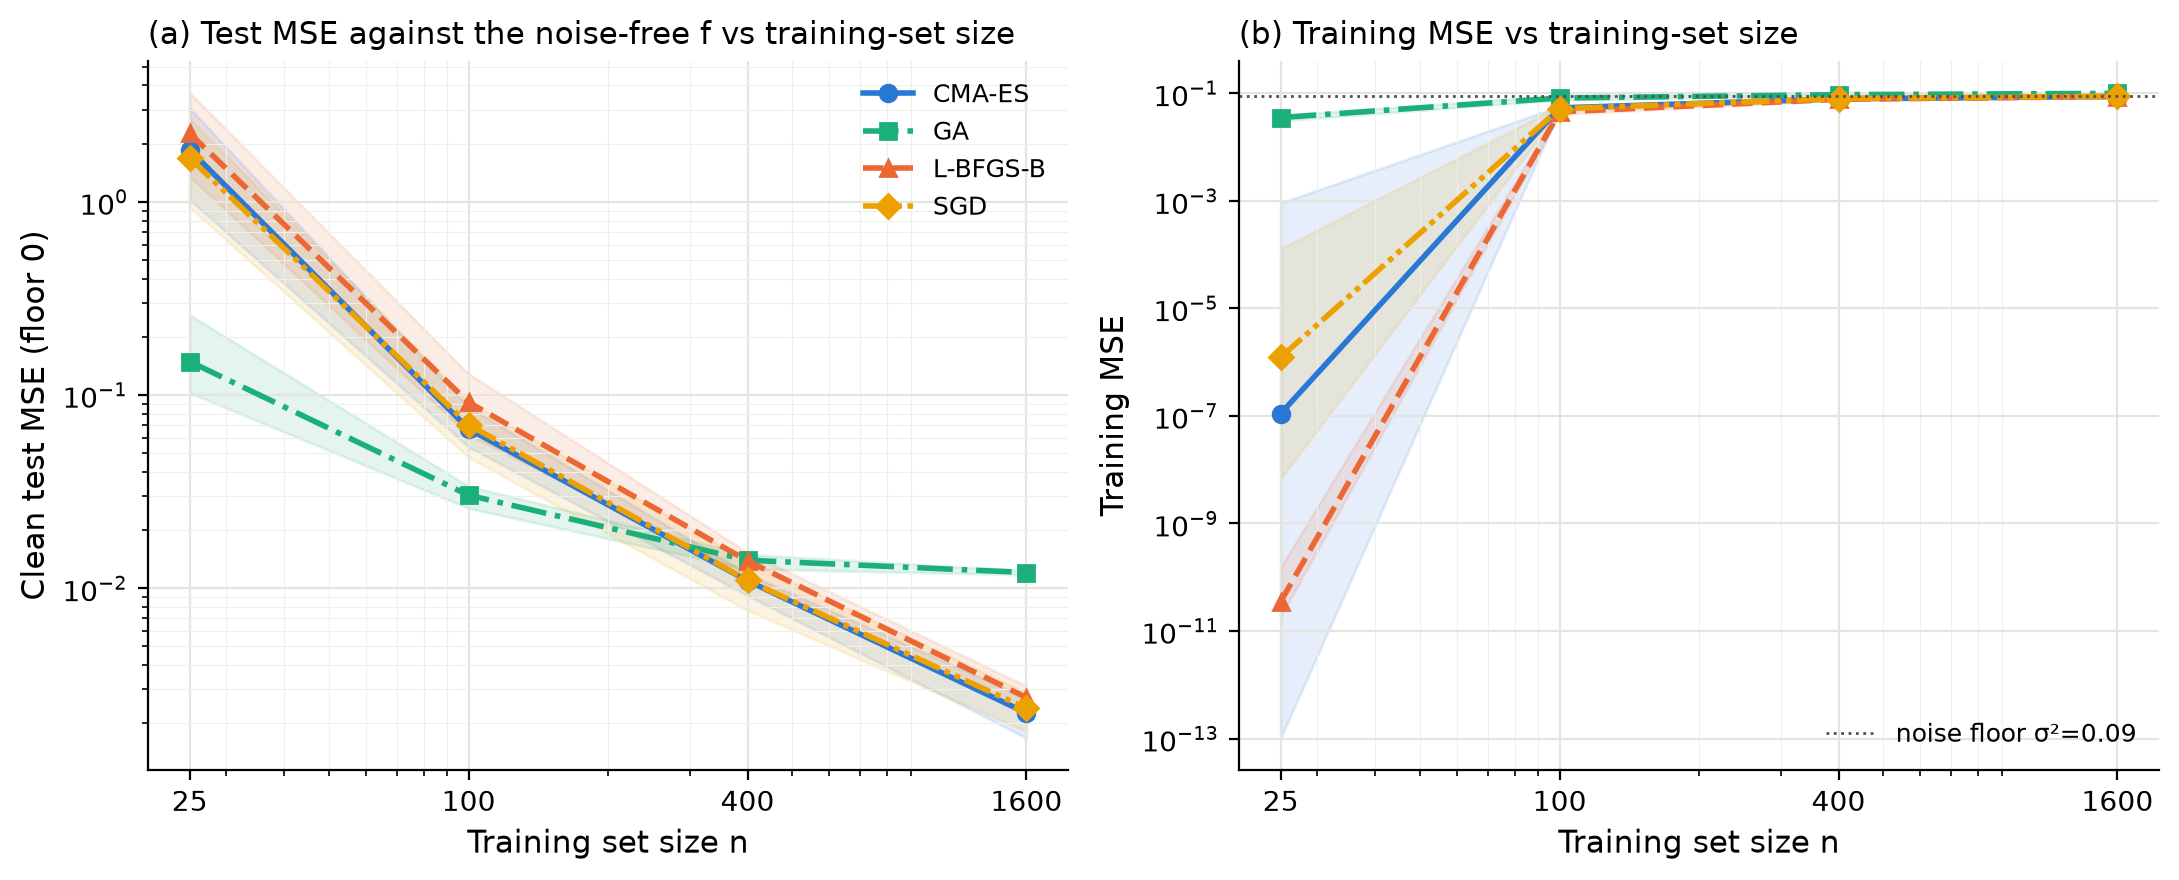
\includegraphics[width=\textwidth]{fig1_test_train_vs_n.png}
  \caption{Core sweep: clean test MSE (left) and training MSE (right) vs.\ $n$ (median and IQR,
  log--log). Dotted line: noise floor $\nfloor=0.09$.}
  \label{fig:core}
\end{figure}

At $n\le100$, the GA beats every other method (Cliff's $\hat\delta\approx0.95$--$0.98$,
$p_{\mathrm{Holm}}<10^{-7}$). However, the GA has the highest training MSE at every $n$: its small-$n$
advantage comes with fitting less. At $n=25$ all three gradient-converged methods interpolate the
training data (train MSE $\approx0$) and their clean test MSE is $>17\times$ the noise floor. At
$n\ge400$, \cmaes{} and Adam approach the noise floor; the GA lags behind due to underfitting.
Among the converged methods, \lbfgs{} fits hardest but generalises worst at $n\le400$: fitting
more does not mean generalising better.

\begin{figure}[h]
  \centering
  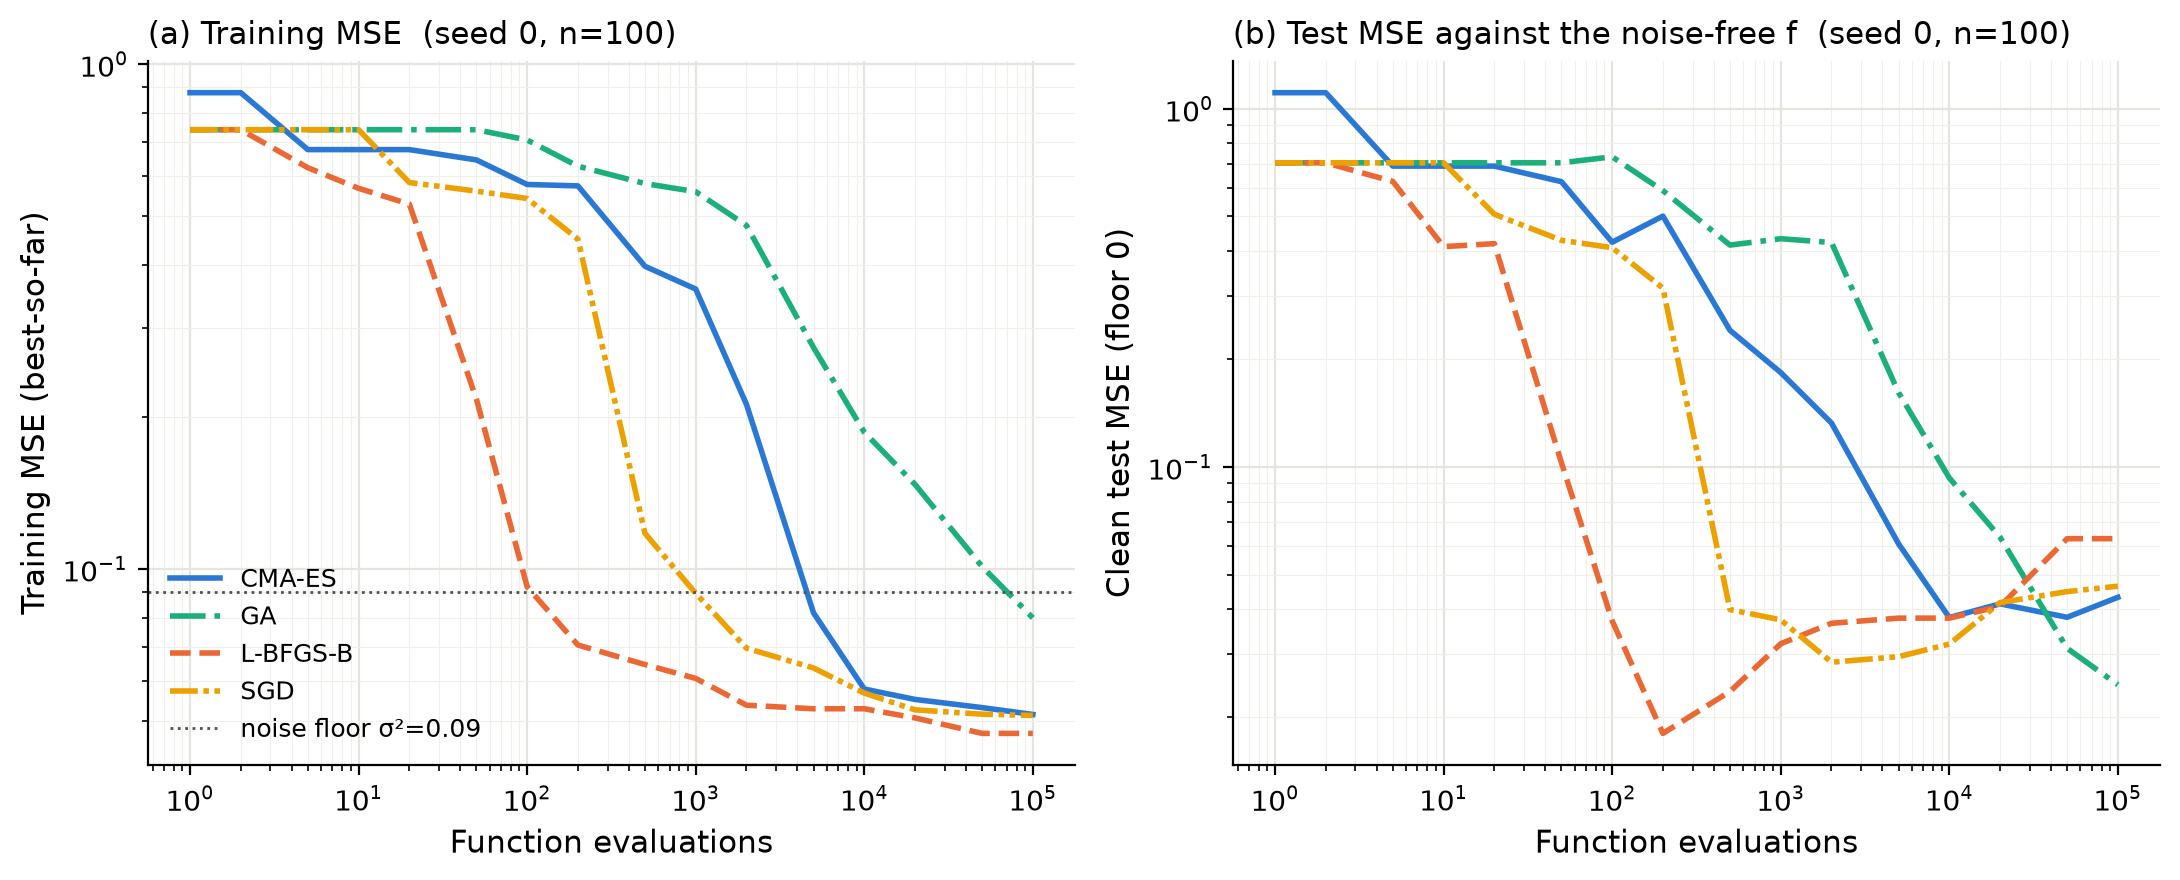
\includegraphics[width=\textwidth]{fig4_convergence_seed0_n100.png}
  \caption{Convergence (seed 0, $n=100$): \lbfgs{} reaches its lowest test error after $\sim$200
  evaluations and then overfits; the GA is still improving on the training set at $10^5$.}
  \label{fig:convergence}
\end{figure}

\subsection{Robustness checks}

\textbf{Ten-fold GA budget.} With $10^6$ evaluations (seeds 0--9) the GA fits more, its large-$n$
disadvantage mostly disappears, and at $n=25$ it starts to overfit (test rises from 0.138 to 0.269,
$p_\mathrm{Holm}=0.008$). It still fits less than the other methods at $n=100$ (train 0.071 vs.\
0.043--0.052): the GA never reaches ``fits as well, generalises better''.

\textbf{Gradient cost.} With $g=1$ or $g=3$, 23 of 24 pairwise verdicts are unchanged; the one
exception is Adam at $n=100$ with $g=3$ ($p_\mathrm{Holm}=0.015$). The choice $g=2$ does not drive the results.

\textbf{Wall-clock budget.} With per-$n$ time limits (4, 4, 7, 12\,s), 19 of 24 verdicts are
unchanged. The GA gets more evaluations per second and catches up at $n=400$.

\subsection{Fair early stopping}

In the core sweep only the GA stops early (it never reaches the overfitting stage). We then gave
every method the same early stopping: for each run we picked the checkpoint with the lowest MSE on
an independent selection set of $n$ points drawn per seed (Table~\ref{tab:es}). The GA's small-$n$ advantage disappears: at $n=100$ no method differs
from the best (\lbfgs), but Adam beats the GA ($p_\mathrm{Holm}=0.011$); at $n\ge400$ the GA is
the worst. The gradient methods reach their best networks very early (\lbfgs{} after 100--500
evaluations, Adam 1.4k--4k, \cmaes{} 4k--20k); the GA needs the whole budget for $n\ge100$.

\begin{table}[h]
  \centering
  \caption{Early stopping on a selection set of $n$ points (30 seeds): median clean test MSE /
  median evaluations at the selected checkpoint. \textbf{Bold}: not significantly worse than the best.}
  \label{tab:es}
  \small
  \begin{tabular}{@{}r cccc@{}}
    \toprule
    $n$ & \cmaes & GA & \lbfgs & Adam \\
    \midrule
    25   & \textbf{0.129} / 4.0k  & \textbf{0.116} / 20k  & \textbf{0.117} / 100 & \textbf{0.148} / 1.4k \\
    100  & \textbf{0.032} / 10k   & \textbf{0.031} / 100k & \textbf{0.024} / 158 & \textbf{0.027} / 3.2k \\
    400  & \textbf{0.0052} / 13k  & 0.014 / 100k          & \textbf{0.0057} / 251 & 0.0065 / 4.0k \\
    1600 & \textbf{0.0012} / 20k  & 0.012 / 100k          & \textbf{0.0013} / 500 & 0.0018 / 3.2k \\
    \bottomrule
  \end{tabular}
\end{table}

\begin{figure}[h]
  \centering
  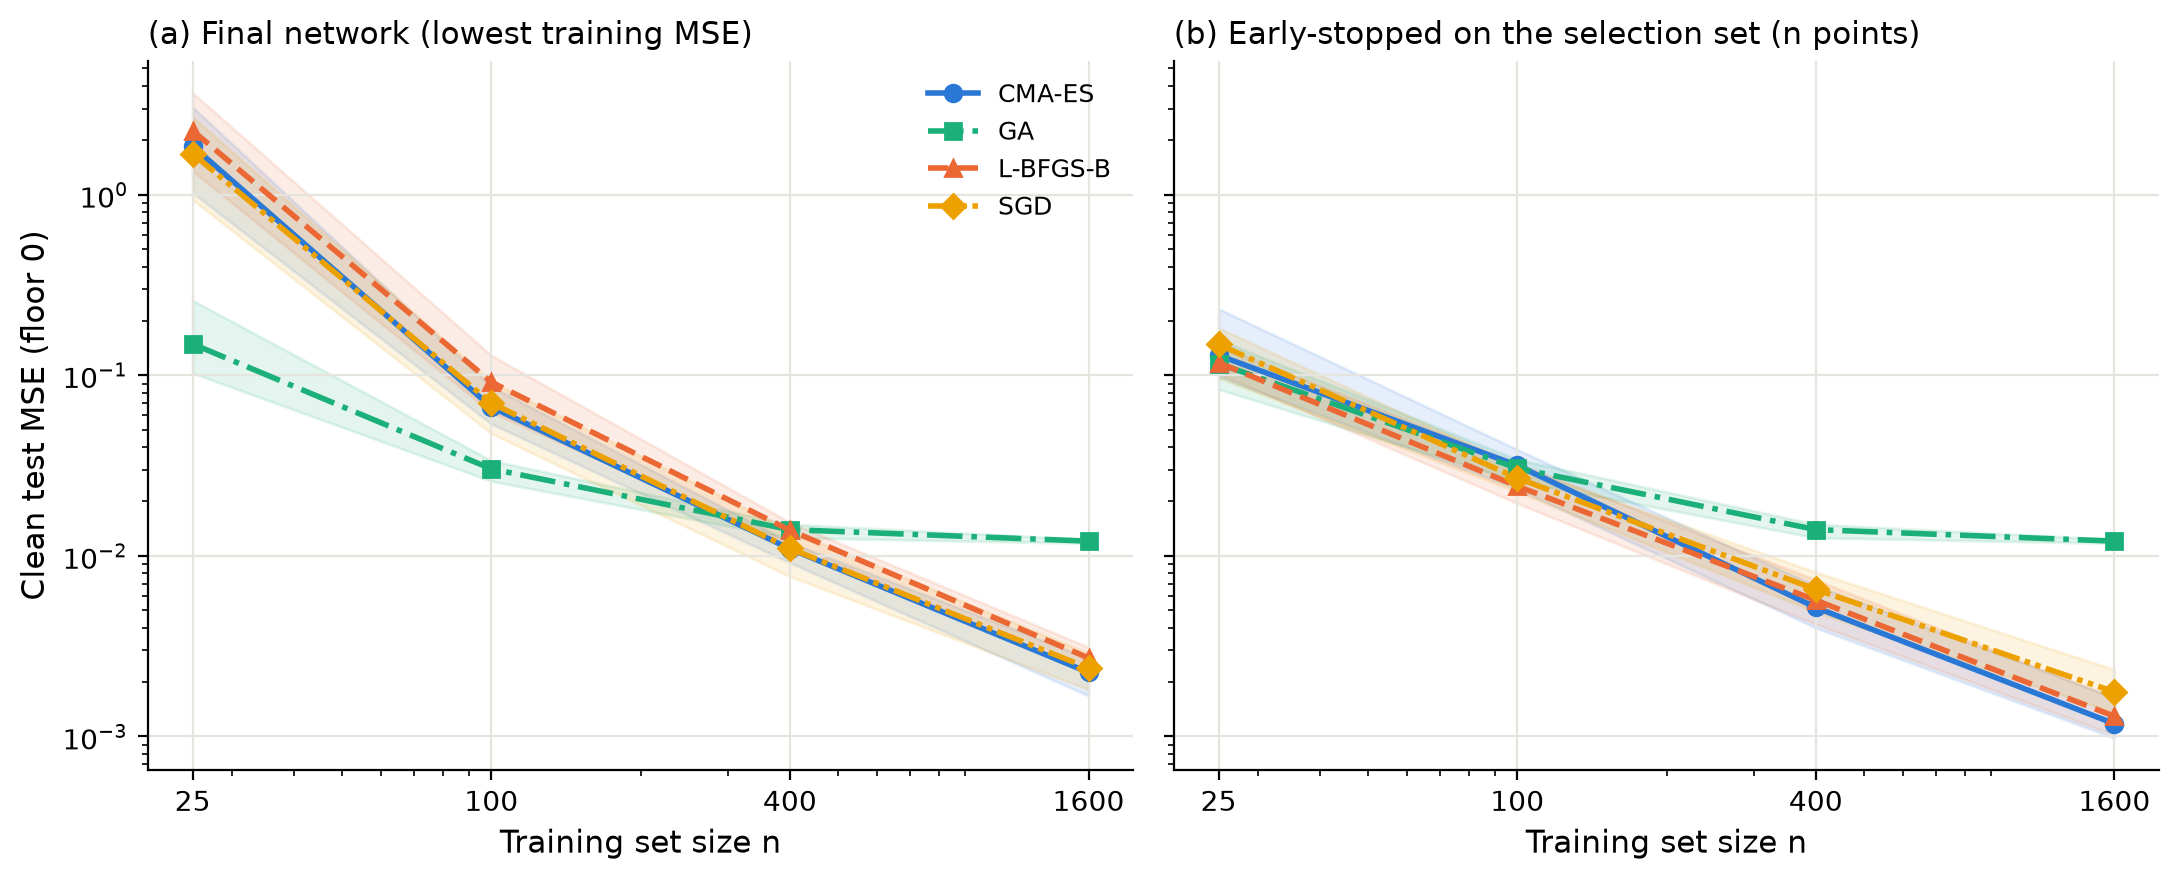
\includegraphics[width=\textwidth]{fig5_early_stopping_vs_n.png}
  \caption{Clean test MSE vs.\ $n$: (a) returned network (lowest training MSE), (b) early-stopped
  on the selection set of $n$ points. The GA's small-$n$ advantage disappears under fair early stopping.}
  \label{fig:es}
\end{figure}

\subsection{Hidden-layer size selection}

We also tested whether each method benefits from choosing $H\in\{2,4,6,10,15,20\}$ on the selection
set. \lbfgs{} and \cmaes{} prefer smaller networks at $n\le400$ ($H=6$--$10$), while the GA
consistently picks the largest ones ($H=15$--$20$), compensating its underfitting with extra capacity.
The ranking does not change, but \lbfgs{} gains the most from capacity selection at $n=100$.

\begin{figure}[h]
  \centering
  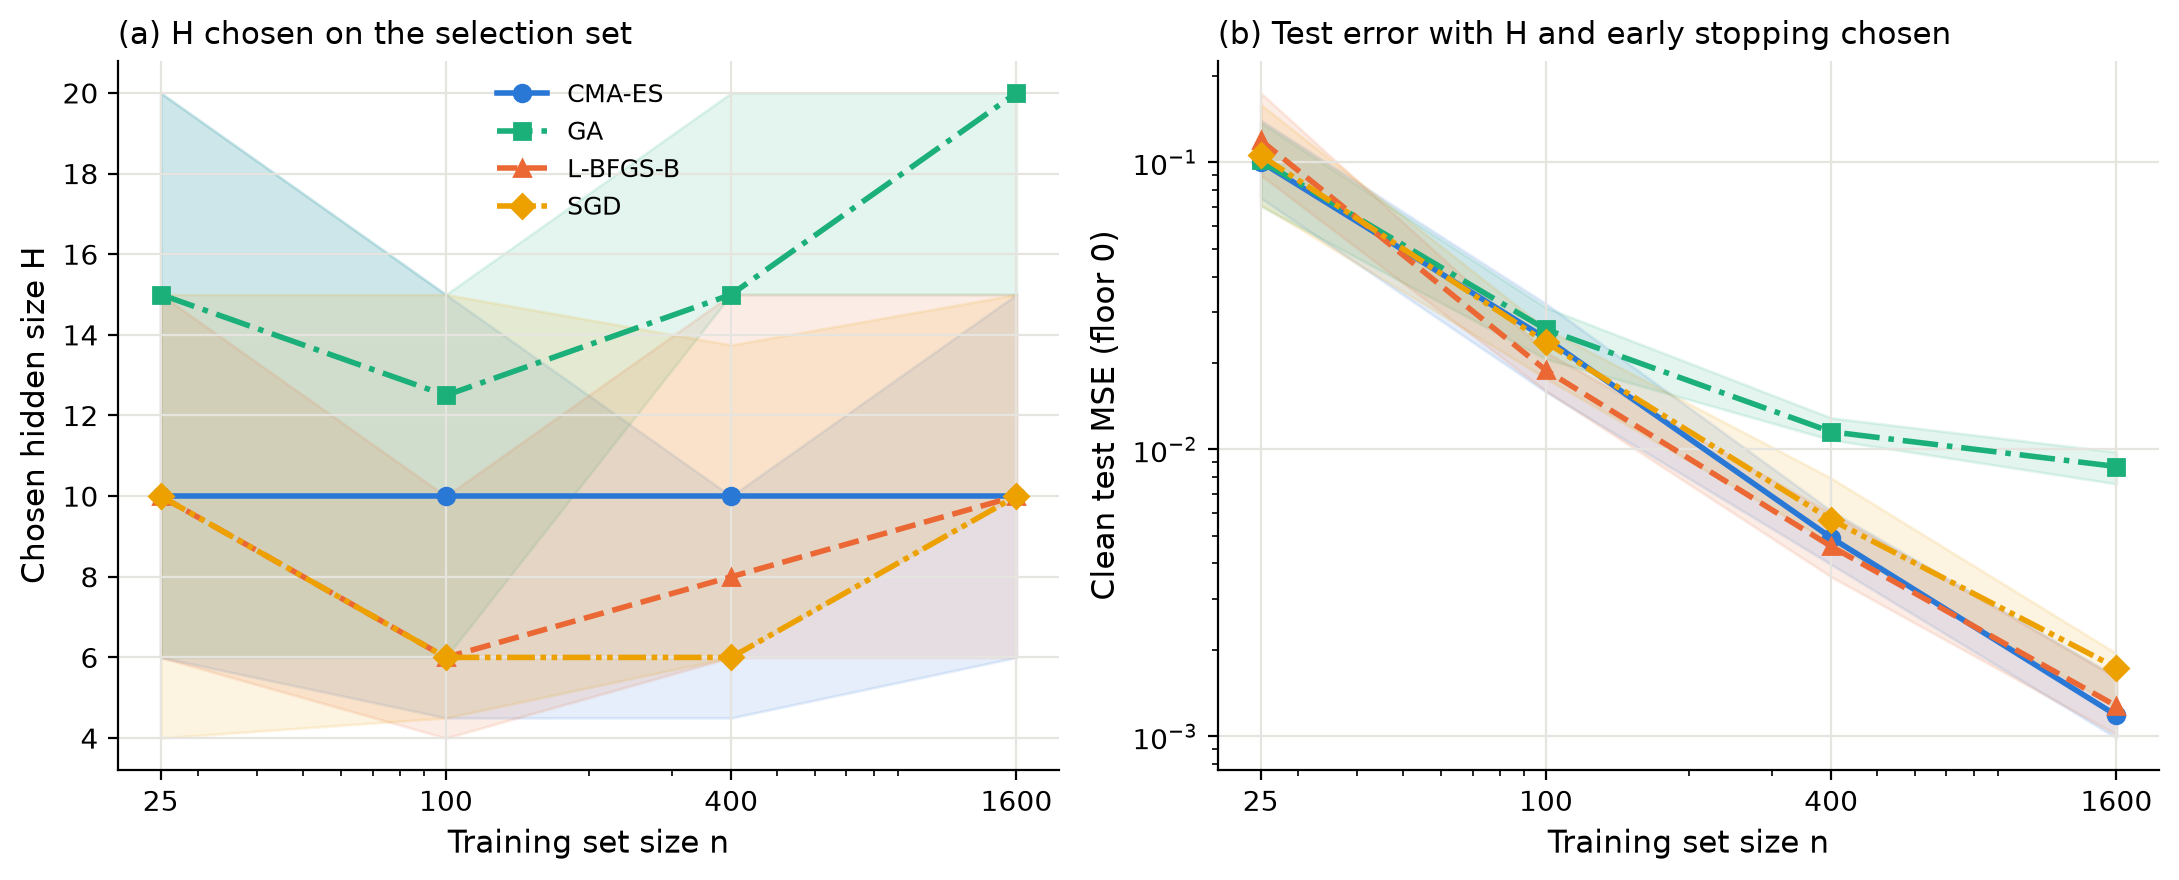
\includegraphics[width=\textwidth]{fig7_chosen_h.png}
  \caption{(a) Hidden size chosen on the selection set and (b) clean test MSE of the chosen networks
  vs.\ $n$. The GA consistently picks the largest networks; \lbfgs{} and \cmaes{} prefer smaller ones
  at small $n$.}
  \label{fig:arch}
\end{figure}

% ============================================================
\section{Mechanism}
\label{sec:mechanism}
% ============================================================
The MLP error landscape is \emph{deceptive} and \emph{multimodal} \citep{yao1999evolving}: gradient
methods get trapped in whichever minimum they find first. The convergence curves
(Figure~\ref{fig:convergence}) show that \lbfgs{} reaches a low training loss in under 1000 evaluations
and then restarts; \cmaes{} improves more gradually. The pilot study (3 seeds) also revealed a
counterintuitive finding: at $n=100$ the clean test MSE of \cmaes{} \emph{rises} with the budget
(0.039 at $10^4$ evaluations $\to$ 0.072 at $10^5$). An under-converged optimiser can look as if it
generalises better --- which is exactly what happens with the GA.

\cmaes{} adapts its step size and learns a full covariance matrix \citep{hansen2001completely},
so it aligns its search with the geometry of the landscape in a way that axis-aligned mutation
(the GA, with $\sigma_{\mathrm{mut}}=0.03$ per gene) cannot. The GA's small step and low mutation
rate mean it makes slow progress and stops --- not at a good minimum, but before it reaches one.

The sharpness measurement confirms this. We define perturbation sharpness as
$S_\rho(\bm\theta) = \frac{1}{K}\sum_{k=1}^{K}[\Ltr(\bm\theta+\bm\epsilon_k)-\Ltr(\bm\theta)]$
where $K=200$ random directions $\bm\epsilon_k$ have norm $\rho\|\bm\theta\|$, $\rho=0.01$.
To remove the effect of training progress, we compare methods at \emph{matched training error}
(the GA's final training MSE per seed).

\textbf{Sharpness results.} The GA is flatter than \lbfgs{} at every $n$
($p_\mathrm{Holm}\le4\cdot10^{-5}$), but flatness does not predict test error: at $n\ge100$ the
sharpest method (\lbfgs) has the \emph{lowest} test MSE of the matched networks. Only at $n=25$ do
the flatter networks also generalise better. So H1 as a flat-minima story is not supported --- at least
not for the range of $n$ where the data is sufficient for the comparison to be meaningful.

\begin{figure}[h]
  \centering
  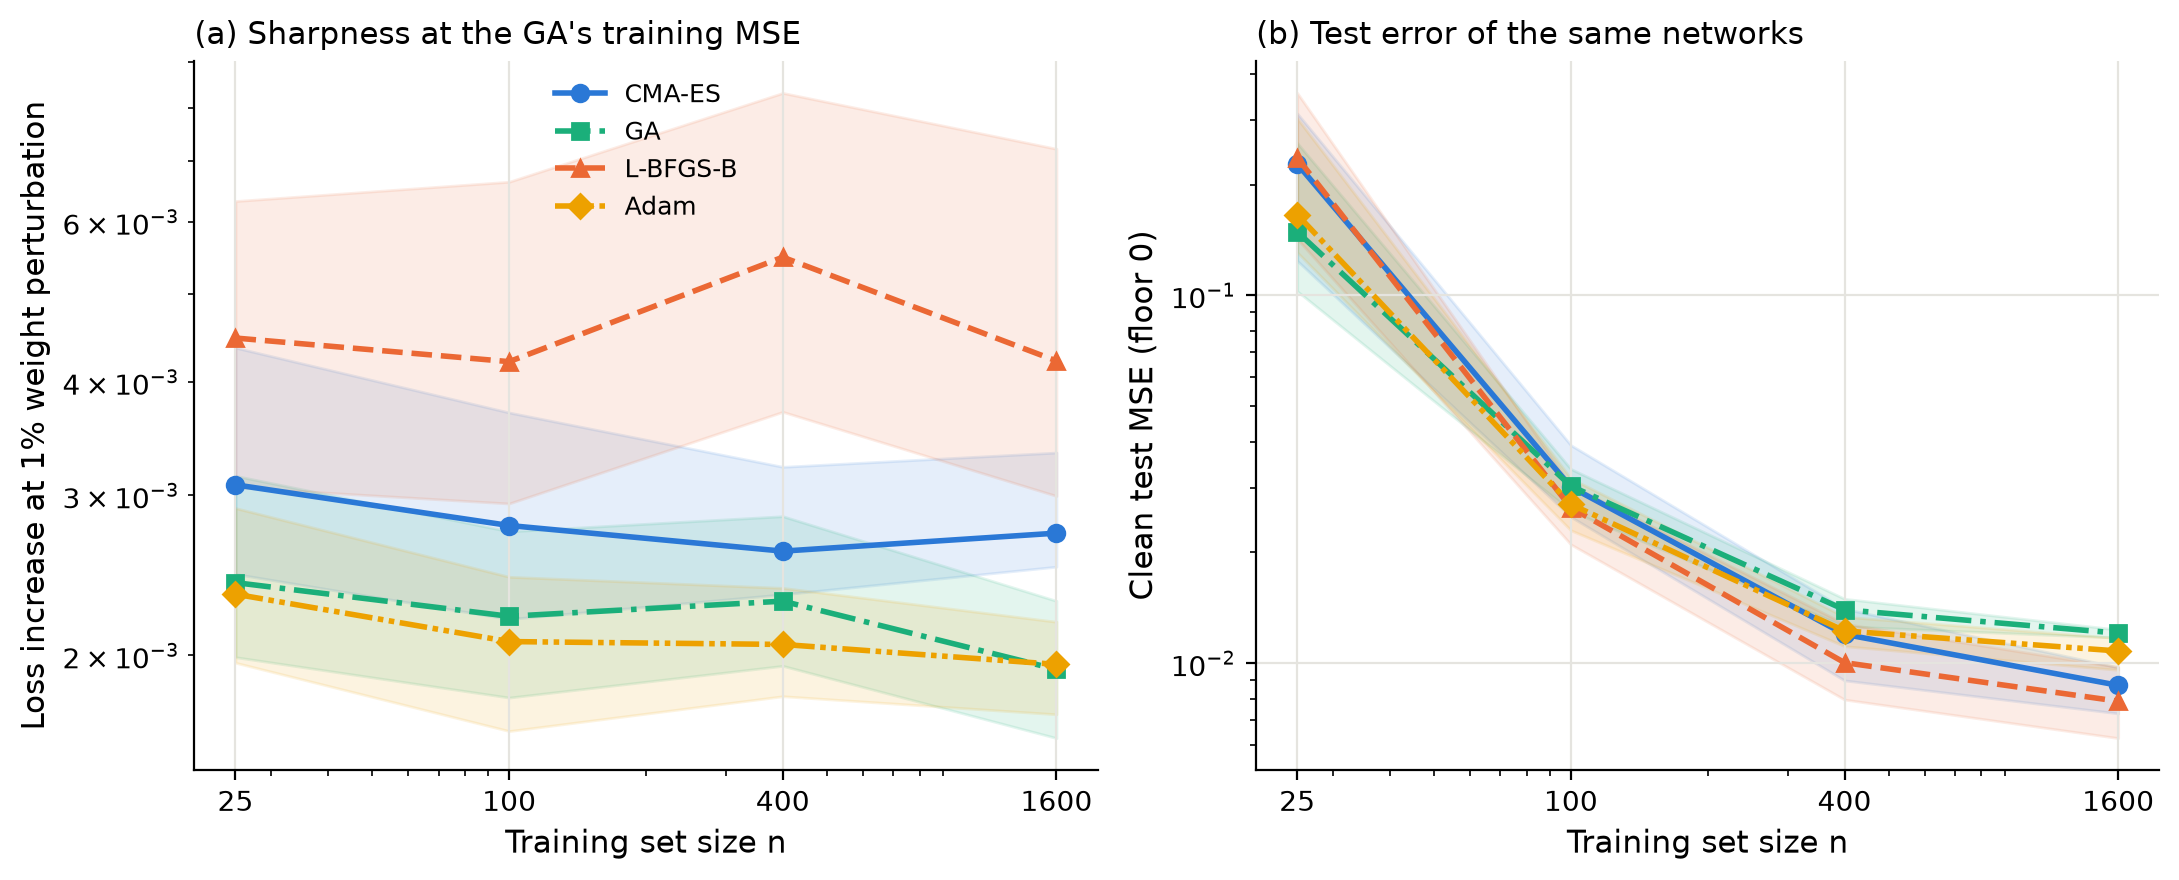
\includegraphics[width=\textwidth]{fig6_sharpness_matched.png}
  \caption{At matched training MSE (the GA's, per seed): (a) perturbation sharpness $S_{0.01}$ and
  (b) clean test MSE of the same networks. The GA is flatter than \lbfgs{} but flatness does not
  predict generalisation at $n\ge100$.}
  \label{fig:sharp}
\end{figure}

\textbf{Bounds.} L-BFGS, \cmaes{} and Adam place 5--17\% of weights at $\pm5$; the GA places almost
none. The bounds act as an implicit regulariser for the converged methods; the GA, which never reaches
them, does not benefit from this effect.

% ============================================================
\section{Limitations}
% ============================================================

\textbf{Sharpness is measured in one way only.} We use perturbation sharpness
$S_{0.01}$ with $K=200$ random directions. This is not the Hessian, and we
have not verified that $S_{0.01}$ measures the same thing as the sharpness in
\citet{keskar2017large}, whose measure is scale-dependent. The conclusion that
H1 is not a flat-minima story rests on this single measure.

\textbf{One problem, one noise level.} All results come from one smooth 2-D
function with $\sigma=0.3$. If the GA's advantage is implicit early stopping,
it is not clear whether it would grow or shrink with higher noise --- that
depends on whether more noise makes it harder to overfit, which we did not test.

\textbf{The GA has not converged at $10^5$ evaluations.} The GA's training MSE
is still falling 7--9\% over the second half of the budget at $n\ge100$. Its
results in the core sweep measure ``fits less'' rather than ``generalises
better''. With $10^6$ evaluations it converges at $n\ge400$ (test MSE
$0.015\to0.007$ at $n=400$; $0.012\to0.003$ at $n=1600$), but it still fits
less than the other methods at every $n$ (train MSE $0.071$ vs.\ $0.043$--$0.052$
at $n=100$). The GA's best mutation step ($\sigma_{\mathrm{mut}}=0.03$) was at
the edge of the tuning grid and was not extended further; a wider search might
help, but we did not test it.

\textbf{Statistical power of the long GA run.} The 1M-evaluation GA run uses
only 10 seeds. With 10 seeds the minimum achievable $p_{\mathrm{Holm}}$ over
24 tests is $\approx0.047$, so the comparisons in that column are descriptive
only (effect sizes, no significance claims).

\textbf{Weight bounds act differently across methods.} The bounds $[-5,5]$ act
as an implicit regulariser for \cmaes, \lbfgs{} and Adam (5--17\% of weights
at the bounds), but not for the GA ($\approx0\%$). This is a confound we
measured but did not control for.

\textbf{Environment.} \cmaes{} did not reproduce bit-for-bit across machines
(\texttt{cma}/numpy version matters). The conclusions held on both machines.

% ============================================================
\section*{Use of AI Tools}
\addcontentsline{toc}{section}{Use of AI Tools}
% ============================================================

During this project we used OpenCode (powered by Claude Sonnet, Anthropic) and Claude (Anthropic)
as AI assistants for the following tasks:

\begin{itemize}
  \item Summarising and contextualising the relevant literature, which we used to motivate the
        research question and hypothesis.
  \item Drafting and iteratively refining all sections of this report. We reviewed and corrected
        each section against our experimental data.
  \item Assisting with parts of the implementation: \texttt{scripts/aggregate\_results.py},
        \texttt{scripts/make\_figures.py}, and \texttt{README.txt}.
  \item Formatting the title page, header and table of contents in \LaTeX.
\end{itemize}

All experimental decisions are documented in \texttt{docs/PROJECT\_PLAN.md}. The conclusions drawn
from the results are our own.

% ============================================================
\addcontentsline{toc}{section}{References}
\bibliographystyle{abbrvnat}
\bibliography{references}
% ============================================================

\end{document}
